% Inicializa o documento
% define papel, tamanho global de fonte, tipo de documento
\documentclass[a4paper, twoside, 12pt]{article}

	% Pacotes usados
	\usepackage[utf8]{inputenc} % enconding de caracteres
	\usepackage[brazil]{babel}  % locale pt_BR
	\usepackage[lmargin=2cm, rmargin=2cm, tmargin=2cm, bmargin=2cm]{geometry} % margens da folha
	\usepackage{indentfirst} % sempre indenta o primeiro parágrafo

	% Matemática	
	\usepackage{amsmath}
	\usepackage{amsfonts}
	\usepackage{gensymb}
	
	% Para links e url
	\usepackage[hidelinks]{hyperref}
	
	\usepackage{listings} % listagem de código-fonte
	\renewcommand*{\lstlistingname}{Listagem} % texto para listagem de código
	\usepackage{color} % cor para usar na listagem de código-fonte
	\usepackage{svg}
	\usepackage{graphicx,xcolor} % para inserir imagens
	\usepackage[nottoc,notlot,notlof]{tocbibind} % adiciona o tópico Referências ao Sumário
	\usepackage{textcomp} % accesso \textquotesingle

	% Para desenhar grafos
	\usepackage{tikz}
	\usetikzlibrary{arrows,positioning,shapes,decorations}

	% Desenhar circulos
	\usepackage{tkz-euclide}
	\usetkzobj{all}

	% Escrever algoritmos em pseudo-código
	\usepackage[portuguese,linesnumbered,ruled]{algorithm2e}

	% Tabelas
	\usepackage{booktabs}
	\usepackage{caption}
	
	% Lista
	\usepackage[shortlabels]{enumitem}

	% Estilos para usar nos grafos
	\tikzset{
		>=stealth',
		punkt/.style={
			rectangle,
			text centered,
			inner sep=0.7em,
			draw,
			fill=blue!5
		},
		pil/.style={
			->,
			thick,
			shorten <=2pt,
			shorten >=2pt
		}
	}

	% Para plotar gráficos
	\usepackage{pgfplots}
	\pgfplotsset{width=10cm,compat=1.9}

	% Define cores para o highlight de código-fonte
	\definecolor{dkgreen}{rgb}{0,0.6,0}
	\definecolor{gray}{rgb}{0.5,0.5,0.5}
	\definecolor{mauve}{rgb}{0.58,0,0.82}
	
	% Define configuração para listagem de código-fonte em linguagem C
	\lstset{
		frame=tb,
		language=C,
		aboveskip=2mm,
		belowskip=2mm,
		showstringspaces=false,
		columns=flexible,
		basicstyle={\small\ttfamily},
		numbers=none,
		keywordstyle=\color{blue},
		commentstyle=\color{dkgreen},
		stringstyle=\color{mauve},
		breaklines=true,
		breakatwhitespace=false,
		tabsize=4
	}

% Começo do documento
\begin{document}

	% Define algum espaçamento que eu não lembro, hehe :)
	\setlength\parskip{0.3cm}

	% Insere a Capa
	% Começo da folha de Capa
\begin{titlepage}

		% Título
		\title{
\textsc {\large Universidade de São Paulo\\
Instituto de Ciências Matemáticas e de Computação}\\[1cm]
{\large SCC0205 -- Teoria da Computação e Linguagens Formais}\\[5cm]
{\LARGE Trabalho 1 -- Analisador Léxico e Sintático para Linguagem AWK\\[4cm]}
		}

		% Autores
		\author{
Elias Italiano Rodrigues -- 7987251\\
Gabriel Tessaroli Giancristofaro -- 4321350\\
Paulo Augusto de Godoy Patire -- 7987060
		}

		% Inserção manual de data
		\date{
\vfill São Carlos, 2 de outubro de 2014
		}

		% Cria a Capa
		\maketitle
		\thispagestyle{empty}

% Fim da folha de Capa
\end{titlepage}

	
	% Reseta contador de página para 1 (assim não conta a Capa como página)
	\setcounter{page}{1}
	
	% Insere as outras partes do documento
	% Cria o Sumário
\tableofcontents

% Cria uma nova página, forçando o Sumário a ficar numa página separada
\newpage


	\section{Introdução \label{sec:introducao}}

Este trabalho implementa um analisador semântico com tratamento de erros para a linguagem de programação \texttt{LALG} utilizando as ferramentas \texttt{flex} e \texttt{bison}. Foram seguidas as instruções dadas em sala de aula assim como consultadas em manual~\cite{bib:manual} e em livro~\cite{bib:livro}.

	\section{Soma dos Subconjuntos}

\subsection{Enunciado}

Assim como definido no enunciado do Trabalho 3 da disciplina, o problema é o seguinte:

\textsc{Subset-Sum}: dado um conjunto finito de números naturais $S$ e um valor $t \in \mathbb{N}$, existe algum subconjunto não-vazio $S' \subseteq S$ em que seus elementos somados resultem em $t$?

Ou pode-se definir o problema mais formalmente como uma linguagem:

\textsc{Subset-Sum} $= \{ \langle S, t \rangle$ : existe um subconjunto $S' \subseteq S$ tal que $t = \sum_{s \in S'}s \}$.

Trata-se de um \textbf{problema de decisão}, uma vez que é esperada uma resposta \textit{sim} ou \textit{não}.

\subsection{Explicação}

Pensando em uma linguagem de programação, pode-se imaginar o conjunto $S$ como um vetor de dados \texttt{unsigned int} de tamanho \texttt{n}, e procura-se por algum subconjunto dele em que a soma dos valores resulte em um valor de entrada \texttt{t}.

\begin{figure}[h]
	\centering
	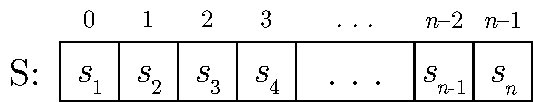
\includegraphics[scale=0.9]{./input/vetor.pdf}
	\caption{Ilustração de um vetor para o conjunto $S$. \label{fig:vetor}}
\end{figure}

Pode-se observar que há uma grande quantidade de subconjuntos para o vetor \texttt{S} em função do seu tamanho \texttt{n}, pois o total de subconjuntos é:

$$
	\sum_{i=1}^{n} {n \choose i} = {n \choose 1} + {n \choose 2} + \cdots + {n \choose n-1} + {n \choose n} = 2^n - 1
$$

Ou seja, é o número de subconjuntos com 1 elemento, mais o número de subconjuntos com 2 elementos etc, até o último subconjunto que é quando $S' = S$, e desconsiderando o conjunto vazio quando $i = 0$.

Dado esse total de subconjuntos possíveis, no pior caso, para encontrar um subconjunto que satisfaça o \textsc{Subset-Sum} e responda \textit{sim}, um algoritmo ingênuo teria complexidade exponencial de $O(2^n)$, pois verificaria todos eles. Por exemplo, um conjunto $S$ de tamanho $n = 100$ tem $2^{100} - 1 = 1\ 267\ 650\ 600\ 228\ 229\ 401\ 496\ 703\ 205\ 375$ subconjuntos não-vazios.


	\newpage
\section{Provas}

\subsection{\textsc{Subset-Sum} está em \textbf{NP}}

Dado que \textbf{NP} é o conjunto dos problemas de decisão em que uma possível solução pode ser verificada em tempo polinomial, para mostrar que \textsc{Subset-Sum} está em \textbf{NP} para uma instância $\langle S, t \rangle$ do problema, toma-se o subconjunto $S'$ para ser verificado. O Algoritmo~\ref{alg:check} de verificação pode checar se $\sum_{s \in S'} s = t$ em tempo polinomial $O(n)$.

\begin{algorithm}[h]
	\KwIn{$\langle S', t \rangle$}
	\KwOut{\textit{true} se $S'$ é solução, \textit{false} caso contrário}

	$sum \leftarrow 0$\;
	\ForEach{$s \in S'$}{
		$sum \leftarrow sum + s$\;
	}
	\If{$sum = t$}{
		\Return{true}\;
	}
	\Return{false}\;
\caption{Verifica uma solução $S'$ do \textsc{Subset-Sum} em tempo polinomial. \label{alg:check}}
\end{algorithm}

\subsection{\textsc{Subset-Sum} é \textbf{NP}-\textit{completo}}

\subsubsection{Redução}

Antes de provar a \textbf{NP}-\textit{completude} do \textsc{Subset-Sum}, é necessário conhecer os problemas canônicos usados para prová-lo por \textbf{redução}.

A técnica de provar por redução que um problema $B$ é \textbf{NP}-\textit{completo}, requer conhecer um problema $A$ que já foi provado ser \textbf{NP}-\textit{completo} e então encontrar uma maneira de reduzir $A \rightarrow B$ ``refraseando'' $A$ ou encontrando um algoritmo que converta qualquer instância de $A$ em uma instância de $B$ em tempo polinomial. Assim, pode-se dizer que $B$ é tão difícil quanto $A$, ou ainda, que $B$ não é mais do que um fator polinomial difícil do que $A$.

Ou seja, se $A \leq_{\textbf{P}} B$ e $A \in$ \textbf{NP}-\textit{completo} $\Rightarrow$ $B \in$ \textbf{NP}-\textit{completo}.

\subsubsection{Problemas de Satisfatibilidade Conhecidos}

\textbf{\textsc{Circuit-Sat}} é um problema canônico de satisfatibilidade provado pertencer a \textbf{NP}-\textit{completo}. Seu enunciado é: dado um circuito booleano combinacional, ele é satisfatível?

Ou, mais formalmente como uma linguagem:
	
\textsc{Circuit-Sat} $ = \{ \langle C \rangle$ : $C$ é um circuito booleano combinacional satisfatível $\}$.

Um circuito booleano combinacional é um conjunto de variáveis que podem receber os valores 0 (\textit{false}) ou 1 (\textit{true}) e que de acordo com as operações lógicas AND ($\land$), OR ($\lor$) e NOT ($\lnot$) pode resultar em uma resposta 0 ou 1. Dado um circuito $C$, pode-se determinar se ele é satisfatível simplesmente testando todas as atribuições possíveis para suas $n$ variáveis, que é um total de $2^n$ atribuições.

O \textsc{Circuit-Sat} foi provado ser \textbf{NP}-\textit{completo}, pois, tratando-o mais abstratamente como uma linguagem $L \subseteq \{0,1\}^*$, satisfaz as seguintes propriedades:
\begin{enumerate}[itemindent=1cm]
	\item $L \in \textbf{NP}$, e 
	\item $L' \leq_{\textbf{P}} L$ para todo $L' \in \mathbf{NP}$.
\end{enumerate}

\textbf{\textsc{SAT}} é um problema de decidir se uma fórmula booleana $\phi$ é satisfatível.

Como linguagem:
\textsc{SAT} $= \{ \langle \phi \rangle$ : $\phi$ é uma fórmula booleana satisfatível $\}.$
	
Um fórmula booleana, além dos operadores $\land$, $\lor$, $\lnot$, contém também $\implies$ (implicação) e $\iff$ (se e somente se). O problema \textsc{Circuit-Sat} pode ser reduzido ao \textsc{SAT} e logo também \textsc{SAT} pertence a \textbf{NP}-\textit{completo}.

\textbf{\textsc{3-CNF-SAT}} é um problema de decidir se uma fórmula booleana $\phi$ em 3-CNF é satisfatível.

Como linguagem:
\textsc{3-CNF-SAT} $= \{ \langle \phi \rangle$ : $\phi$ é uma fórmula booleana 3-CNF satisfatível $\}.$

A 3-CNF -- Forma Normal Conjuntiva com 3 literais -- é uma maneira canônica de expressar uma fórmula booleana como uma conjunção de disjunções em que cada cláusula tem exatamente 3 literais -- um literal é a ocorrência de uma variável ou de sua negação. Por exemplo, a seguinte fórmula é 3-CNF: $(x_1 \lor \lnot x_3 \lor \lnot x_2) \land (x_3 \lor x_2 \lor x_4) \land (\lnot x_1 \lor \lnot x_3 \lor \lnot x_4)$. Seguindo o diagrama da Figura~\ref{fig:sat}, o \textsc{3-CNF-SAT} é provado ser \textbf{NP}-\textit{completo} por redução do \textsc{SAT}.

A prova de \textbf{NP}-\textit{completude} dos problemas citados nesta Seção está fora do escopo deste trabalho, mas seu conhecimento é necessário para ser usado na prova de \textbf{NP}-\textit{completude} do \textsc{Subset-sum}.

\begin{figure}[h]
	\centering
	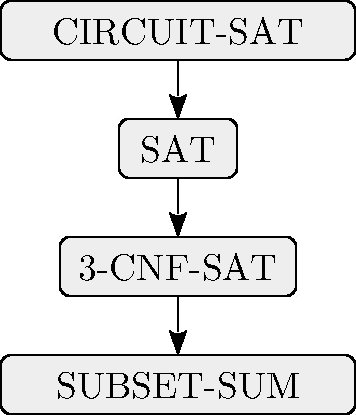
\includegraphics[scale=0.7]{./input/sat.pdf}
	\caption{Dependência de problemas para a prova de \textbf{NP}-\textit{completude} do \textsc{Subset-Sum}. \label{fig:sat}}
\end{figure}

\subsubsection{\textsc{Subset-Sum} usando \textsc{3-CNF-SAT}}

Dada uma fórmula $\phi$ sobre as variáveis $x_1, x_2, \dots, x_n$ com cláusulas $C_1, C_2, \dots, C_k$ cada uma contendo exatamente três literais distintos, o algoritmo de redução contrói uma instância $\langle S, t \rangle$ do \textsc{Subset-sum} tal que $\phi$ é satisfatível se, e somente se, existe um subconjunto de $S$ cuja soma é exatamente $t$.

Toma-se os devidos cuidados para que $\phi$ não contenha um literal e sua negação em uma mesma cláusula e cada variável de $\phi$ apareça pelo menos uma vez em alguma cláusula.

A redução cria dois números em $S$ para cada variável $x_i$ e dois números em $S$ para cada cláusula $C_j$. Assim construímos $S$ e $t$ da seguinte maneira. Para cada valor $s \in S$, nomeamos cada posição de seus dígitos ou por uma variável ou por uma cláusula de $\phi$. Os $k$ menos significantes dígitos de cada $s$ são nomeados pelas cláusulas e seus $n$ mais significantes dígitos são nomeados pelas variáveis.
	
\begin{itemize}
	\item O valor $t$ tem 1 em cada dígito nomeado por uma variável e 4 em cada dígito nomeado por uma cláusula.
	
	\item Para cada variável $x_i$, o conjunto $S$ contém dois inteiros $v_i$ e $v'_i$. Cada $v_i$ e $v'_i$ tem 1 no dígito nomeado por $x_i$ e 0 nos demais dígitos de variáveis. Se o literal $x_i$ aparece numa cláusula $C_j$, então o dígito nomeado por $C_j$ em $v_i$ contém 1. Se o literal $\lnot x_i$ aparece numa cláusula $C_j$, então o dígito nomeado por $C_j$ em $v'_i$ contém 1. Todos demais dígitos nomeados por cláusula em $v_i$ e $v'_i$ são 0.\\
	Dessa maneira, tomado os devidos cuidados citados acima para a fórmula $\phi$, todos os $v_i$ e $v'_i$ são únicos.
	
	\item Para cada cláusula $C_j$, o conjunto $S$ contém dois inteiros $r_j$ e $r'_j$. Cada $r_j$ e $r'_j$ tem 0 em todos os dígitos que não sejam  aqueles nomeados por $C_j$. Para $r_j$, existe um 1 no dígito de $C_j$ e $r'_j$ tem um 2 neste dígito. Esses inteiros são usados para fazer somar até 4 nos dígitos nomeados por cláusulas.
\end{itemize}

Essa redução pode ser feita em tempo polinomial. O conjunto $S$ contruído contém $2n + 2k$ valores $s$, cada um contendo $n + k$ dígitos, e o tempo para produzir cada dígito é $O(n + k)$. O valor $t$ também tem $n + k$ dígitos e também é produzido em tempo polinomial.

Mostra-se agora que a fórmula $\phi$ é satisfatível se, e somente se, existe um $S' \subseteq S$ para os $S$ e $t$ construídos. Primeiro, suponha que existe uma atribuição que satisfaça $\phi$. Para cada $i = 1, 2, \dots, n$, se $x_i = 1$ nessa atribuição, então inclui-se $v_i$ em $S'$. Caso contrário, inclui-se $v'_i$. Dessa maneira, a soma de todos os valores incluídos em $S'$ até agora satisfazem os primeiros $n$ dígitos de $t$. E, para atingir os dígitos 4 de $t$, inclui-se os subconjuntos não-vazios apropriados de variáveis $\{r_j, r'_j\}$ de acordo com as claúsulas $C_j$.

Agora, suponha que existe um subconjunto $S' \subseteq S$ que seus valores some $t$. O subconjunto $S'$ tem que incluir exatamente um $v_i$ ou um $v'_i$ para cada $i = 1, 2, \dots, n$. Caso contrário, os $n$ primeiros dígitos de $t$ não seriam alcançados na soma. E pode-se afirmar que todas claúsulas $C_j$, $j = 1, 2, \dots, n$ também são satisfeitas, pois para alcançar a soma 4 nos $k$ dígitos menos significativos de $t$, o subconjunto $S'$ deve incluir pelo menos um $v_i$ ou um $v'_i$ que tem dígito 1 em $C_j$, e uma vez que as contribuições $r_j$ e $r'_j$ somam no máximo 3, consegue-se totalizar os valores 4 para esses $k$ dígitos.

\newpage
Por exemplo: para $\phi = C_1 \land C_2 \land C_3 \land C_4$, onde $C_1 = (x_1 \lor \lnot x_2 \lor \lnot x_3)$, $C_2 = (\lnot x_1 \lor \lnot x_2 \lor \lnot x_3)$, $C_3 = (\lnot x_1 \lor \lnot x_2 \lor x_3)$ e $C_4 = (x_1 \lor x_2 \lor x_3)$, uma atribuição que satisfaz $\phi$ é $\langle x_1 = 0, x_2 = 0, x_3 = 1 \rangle$. O conjunto $S$ construído pela redução é $S$ = \{ 1001001, 1000110, 100001, 101110, 10011, 11100, 1000, 2000, 100, 200, 10, 20, 1, 2 \} e $t = 1114444$. Como ilustrado na Figura~\ref{fig:reducao}.

\begin{figure}[h]
	\centering
	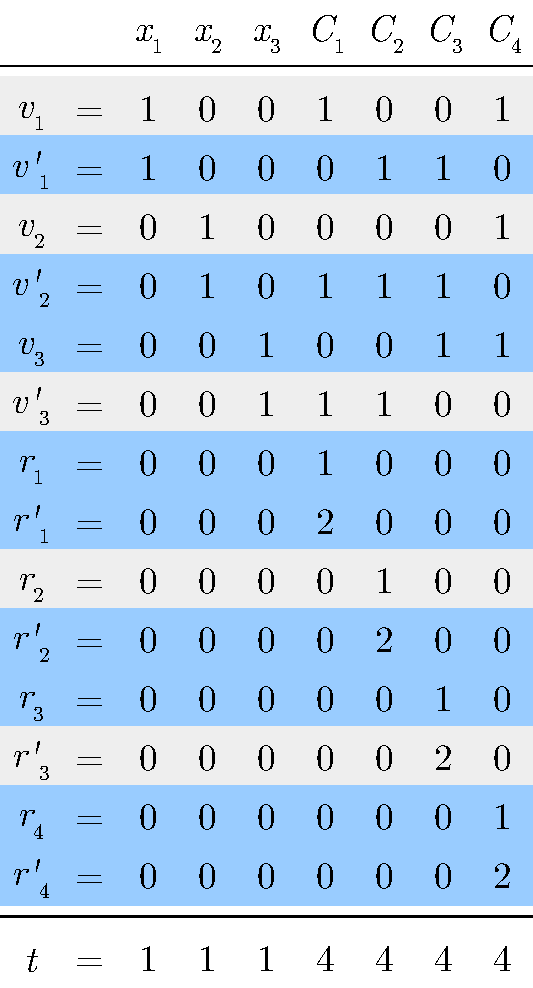
\includegraphics[scale=0.70]{./input/reducao.pdf}
	\caption{Ilustração do conjunto $S$ para uma fórmula $\phi$. As linhas em azul claro são os valores de $S'$ que satisfazem a soma $t$. \label{fig:reducao}}
\end{figure}


	\section{Algoritmos}

\subsection{Exponencial}

Para o Algoritmo~\ref{alg:expo} que responde certamente a pergunta do \textsc{Subset-Sum}, considere que:

\begin{itemize}
	\item Os $n$ elementos de $S$ são numerados ${s_1, s_2, \cdots, s_n}$.

	\item Existe uma função \textsc{Merge-List}$(L, L')$ de complexidade $O(|L| + |L'|)$ que faz a união de duas listas ordenadas $L$ e $L'$ e retorna em uma lista ordenada sem elementos repetidos.
	
	\item A notação $L + s$ denota uma lista com os números de $L$ acrescidos de $s$. Por exemplo, se $L = \{1, 4, 5\}$, então $L + 3 = \{4, 7, 8\}$.
	
	\item Existe uma função \textsc{Search-List}$(L, l)$ de complexidade $O(\log_{2} |L|)$ que busca se um elemento $l$ pertence a lista $L$ e retorna \textit{true} ou \textit{false}.
\end{itemize}

\begin{algorithm}[h]
	\KwIn{$\langle S, t \rangle$}
	\KwOut{\textit{sim} se existe uma solução, \textit{não} caso contrário}
	$n \leftarrow |S|$\;
	$L_0 \leftarrow \{0\}$\;
	\For{$i \leftarrow 1$ \KwTo $n$}{
		$L_i \leftarrow$ \textsc{Merge-List}$(L_{i-1}, L_{i-1} + s_i)$\;
		\If{\textsc{Search-List}$(L_i, t)$}{
			\Return{sim}\;
		}
	}
	\Return{não}\;
\caption{Responde a pergunta do \textsc{Subset-Sum} em tempo exponencial. \label{alg:expo}}
\end{algorithm}

Como o tamanho da lista $L_i$ pode chegar a $2^n$, o Algoritmo~\ref{alg:expo} é em geral de tempo exponencial $O(2^n)$. Para explificá-lo, considere o exemplo dados como entrada $S = \{4, 1, 0, 6, 2\}$ e $t = 7$:
	\begin{align*}
	L_0 & = \{0\} \\
	L_1 & = L_0 \cup L_0 + 4 = \{0, 4\} \\
	L_2 & = L_1 \cup L_1 + 1 = \{0, 1, 4, 5\} \\
	L_3 & = L_2 \cup L_2 + 0 = \{0, 1, 4, 5\} \\
	L_4 & = L_3 \cup L_3 + 6 = \{0, 1, 4, 5, 6, \mathbf{7}, 10, 11\}
	\end{align*}

Então o algoritmo para e retorna \textit{sim}, pois na iteração 4 foi encontrada uma soma para o valor  $t = 7$. Caso nenhuma soma com valor 7 fosse encontrada, no final o algoritmo retornaria \textit{não}.

\subsection{Pseudo-polinomial com Programação Dinâmica}

Em Teoria da Complexidade, um algoritmo executa em tempo pseudo-polinomial se seu tempo de execução é polinomial \textit{no valor numérico} da entrada, mas é exponencial no \textit{comprimento} da entrada -- número de bits requeridos para representá-lo.

No caso do \textsc{Subset-Sum}, pode-se fazer um algoritmo que execute em função do \textit{valor numérico} da soma $max$ de todos os $n$ elementos de $S$.

O Algoritmo~\ref{alg:pseudo} demonstra esse algoritmo pseudo-polinomial usando a técnica de programação dinâmica que armazena os valores já calculados numa matriz (tabela) $Q$ de tamanho $n \times (max + 1)$. Primeiramente é feita uma inicialização da linha 1 de $Q$ e então o algoritmo itera em relação ao valor $max$ para cada outra linha de $Q$.

Como é computado se existe resposta para todos os possíveis valores desde $0$ até $max$, a resposta para $t$ encontra-se na posição $Q(n, t)$ da matriz, mas todas as outras respostas para qualquer valor $0 \leq v \leq max$ encontram-se em $Q(n, v)$.

\SetKw{KwOr}{or}
\begin{algorithm}[h]
	\KwIn{$\langle S, t \rangle$}
	\KwOut{\textit{sim} se existe uma solução, \textit{não} caso contrário}
	
	$n \leftarrow |S|$\;
	$max \leftarrow 0$\;
	
	\For{$i \leftarrow 1$ \KwTo $n$}{
		$max \leftarrow max + s_i$\;
	}
	
	\If{$t < 0$ \KwOr $t > max$}{
		\Return{não}\;
	}
	
	Seja $Q$ uma matriz de tamanho $n \times (max+1)$\;
	\For{$j \leftarrow 0$ \KwTo $max$}{
		$Q(1, j) \leftarrow false$\;
	}
	$Q(1, s_1) \leftarrow true$\;

	
	\For{$i \leftarrow 2$ \KwTo $n$}{
		\For{$j \leftarrow 0$ \KwTo $max$}{
			\uIf{$Q(i-1, j)$ \KwOr $j = s_i$ \KwOr $Q(i-1, j - s_i)$}{
				$Q(i, j) \leftarrow true$\;
			}
			\Else{$Q(i, j) \leftarrow false$\;}
		}
	}
	\If{$Q(n, t)$}{
		\Return{sim}\;
	}
	\Return{não}\;

\caption{Responde a pergunta do \textsc{Subset-Sum} em tempo pseudo-polinomial. \label{alg:pseudo}}
\end{algorithm}


	\section{Aplicações}

O \textsc{Subset-Sum} é um problema muito parecido com o Problema da Mochila (\textsc{Knapsack}) que é um \textbf{problema de otimização} enunciado como: dado um conjunto de $n$ itens $i$, cada um com uma massa $w_i$ e um valor $v_i$, determine quais itens pegar de modo que o total de peso seja menor ou igual a um limite $W$ e o total de valor seja maior ou igual a $K$, desde que não ultrapasse o limite $W$.

Portanto, o \textsc{Subset-Sum} é um caso especial do \textsc{Knapsack}, onde $s_i = v_i = w_i$, $t = K = W$, e logo serve como base para seu entendimento -- inclusive, poderia ser feita a redução \textsc{Knapsack} $\rightarrow$ \textsc{Subset-Sum} para provar sua \textbf{NP}-\textit{completude}. Por sua vez, o \textsc{Knapsack} pode ser aplicado no mundo real para otimização no carregamento de cargas para transporte, empacotamento de produtos, orçamentos e investimentos de capital.

% inkscape -D -z --file=./input/smooth.svg --export-pdf=./input/smooth.pdf

% \begin{figure}[h]
%	\centering
%	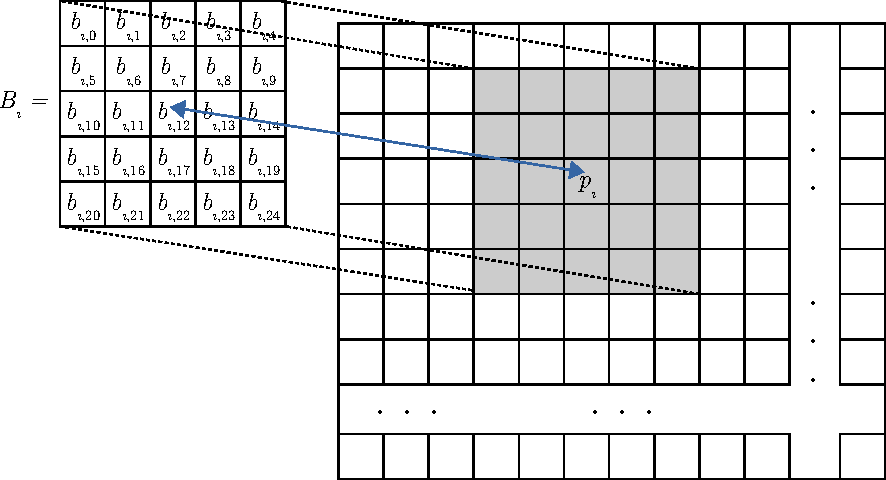
\includegraphics[scale=1]{./input/smooth.pdf}
%	\caption{Ilustração da aplicação de \textit{smooth} em um pixel $p_i$ de uma imagem. \label{fig:ilustracao}}
% \end{figure}


	\section{Conclusão \label{sec:conclusao}}

O trabalho desenvolvido cumpre a especificação dada. Foi possível aprender mais sobre a ferramenta \texttt{flex} e concluir o analisador léxico de \texttt{LALG} que servirá como base para o próximo trabalho.

	\newpage

% Começo das Referências
\begin{thebibliography}{9}

	\bibitem{bib:open-mpi}
		Open MPI\\
		\textless\url{http://www.open-mpi.org/doc/v1.8/}\textgreater\\
		Acesso em: 6 de novembro de 2014.

	\bibitem{bib:cuda}
		Programming Guide :: CUDA Toolkit Documentation\\
		\textless\url{http://docs.nvidia.com/cuda/cuda-c-programming-guide/index.html}\textgreater\\
		Acesso em: 5 de dezembro de 2014.
	
	\bibitem{bib:livro-divisao}
		GRAMA, A. GUPTA, A. KARYPIS, G. and KUMAR, V.\\
		\textit{Introduction to Parallel Computing}. Pearson Education. (2rd ed.). p.101, p.141.

	\bibitem{bib:lena}
		The Lenna Story\\
		\textless\url{http://www.lenna.org/full/len_full.html}\textgreater\\
		Acesso em: 6 de novembro de 2014.

	\bibitem{bib:intro}
		An introduction to the Message Passing Interface (MPI) using C \\
		\textless\url{http://condor.cc.ku.edu/~grobe/docs/intro-MPI-C.shtml}\textgreater
		Acesso em: 9 de novembro de 2014.

% Fim das Referências
\end{thebibliography}

% http://upload.wikimedia.org/wikipedia/commons/8/8f/Whole_world_-_land_and_oceans_12000.jpg


% Fim do documento
\end{document}
